\documentclass[border=10pt]{standalone}
\usepackage{karnaugh-map}
\usepackage{tikz}

\begin{document}
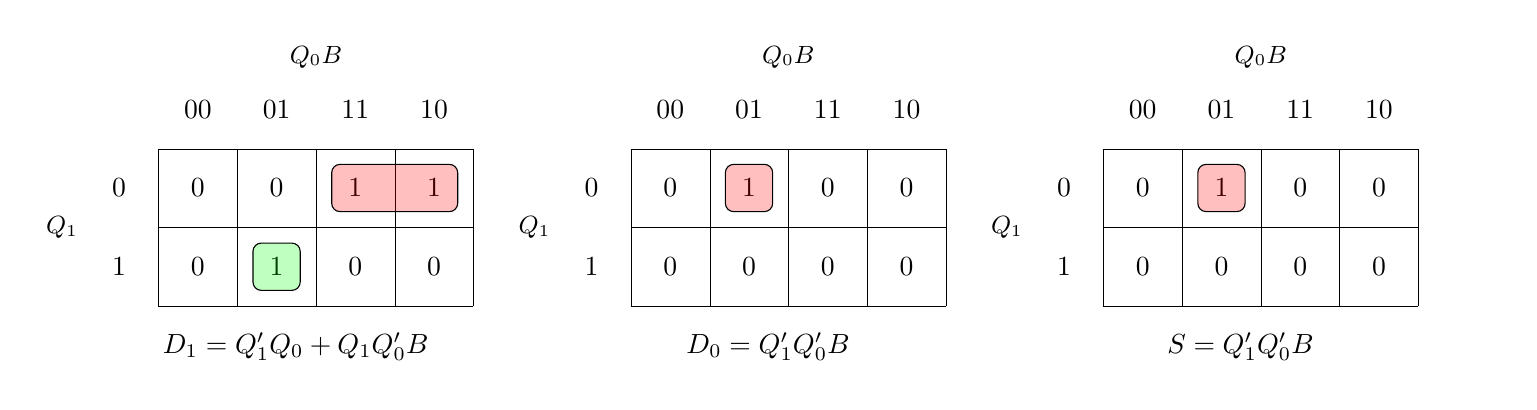
\begin{tikzpicture}
    % Variables: Q1 Q0 B
    % Order: Q1 Q0 (Rows), B (Cols 0, 1)
    
    % D1 (Next Q1)
    % Minterms: 2 (010), 3 (011), 5 (101)
    % Unused (11x -> 6,7) -> 0
    \node at (0, 0) {
        \begin{karnaugh-map}[4][2][1][$B$][$Q_0$][$Q_1$]
            \minterms{2,3,5}
            \autoterms[0]
            \implicant{3}{2} % Q1' Q0
            \implicant{5}{5} % Q1 Q0' B (Isolated?)
            % Check adjacency: 5 (101). Adj: 1 (001-0), 4 (100-0), 7 (111-0), 13?
            % No 5 is isolated 1 on map unless Group with 7 (if X).
            % But unused state 11 is 0. So strict.
        \end{karnaugh-map}
    };
    \node at (0, -1.8) {$D_1 = Q_1' Q_0 + Q_1 Q_0' B$};

    % D0 (Next Q0)
    % Minterms: 1 (001)
    \node at (6, 0) {
        \begin{karnaugh-map}[4][2][1][$B$][$Q_0$][$Q_1$]
            \minterms{1}
            \autoterms[0]
            \implicant{1}{1} % Q1' Q0' B
        \end{karnaugh-map}
    };
    \node at (6, -1.8) {$D_0 = Q_1' Q_0' B$};

    % Output S
    % Minterms: 1 (001)
    \node at (12, 0) {
        \begin{karnaugh-map}[4][2][1][$B$][$Q_0$][$Q_1$]
            \minterms{1}
            \autoterms[0]
            \implicant{1}{1} % Q1' Q0' B
        \end{karnaugh-map}
    };
    \node at (12, -1.8) {$S = Q_1' Q_0' B$};

\end{tikzpicture}
\end{document}
